
% vim: set ts=4 sw=4 tw=80 noexpandtab:
%******************************************************************************%
%                                                                              %
%                   Machine_Learning_04.tex                                    %
%                   Made by: ikourkji                                          %
%                                                                              %
%******************************************************************************%

\documentclass{42-en}

%******************************************************************************%
%                                                                              %
%                                   Prologue                                   %
%                                                                              %
%******************************************************************************%

\begin{document}

\title{Introduction to Machine Learning}
\subtitle{Classification and Logistic Regression}

\member {Jeson}{ljunzhen@42.us.org}
\member {}{Jesonleejunzhen.com}

\summary
{
Learn the most basic type of classification model, logistic regression! 
}

\maketitle

\tableofcontents

%Initialisation des headers d'exercices

\newpage

\bigskip

\centerline{
\includegraphics[width=150mm]{images/dontpanic.png}}

\centerline{\texttt{Eat, Sleep, Code, Repeat.}}

%******************************************************************************%
%                                                                              %
%                           What is Classification?                            %
%                                                                              %
%******************************************************************************%

\chapter{Concepts of Classification}
\section*{What is classification in machine learning?}

Classification is a supervised learning approach in which the computer program learns from the data input given to it and then uses this learning to classify a new observation. This data set may simply be bi-class (like identifying whether the person is male or female or that the mail is spam or non-spam) or it may be multi-class too.\\

One of the most common classification models is logistic regression.

\centerline{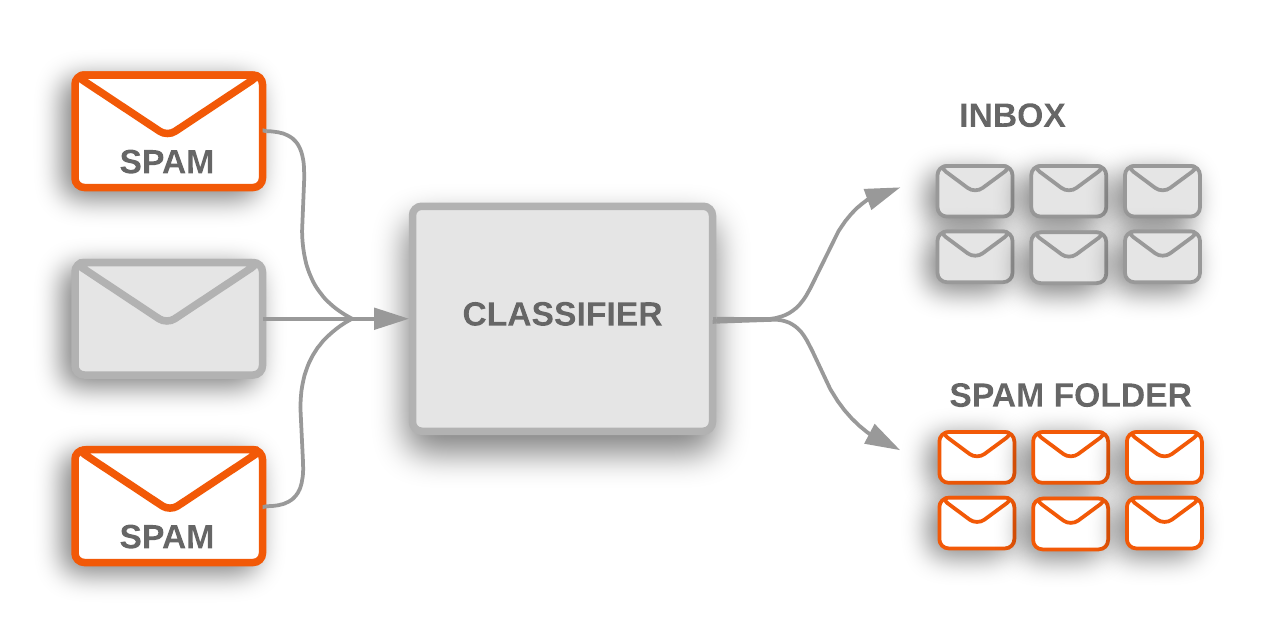
\includegraphics[width=150mm]{images/TextClassificationExample.png}}

\section*{Hypothesis Representation}

Sigmoid Function or also called Logistic Function is one of the functions that can be used to represent our hypothesis for Classification problems(Binary Classification to be exact)\\

\centerline{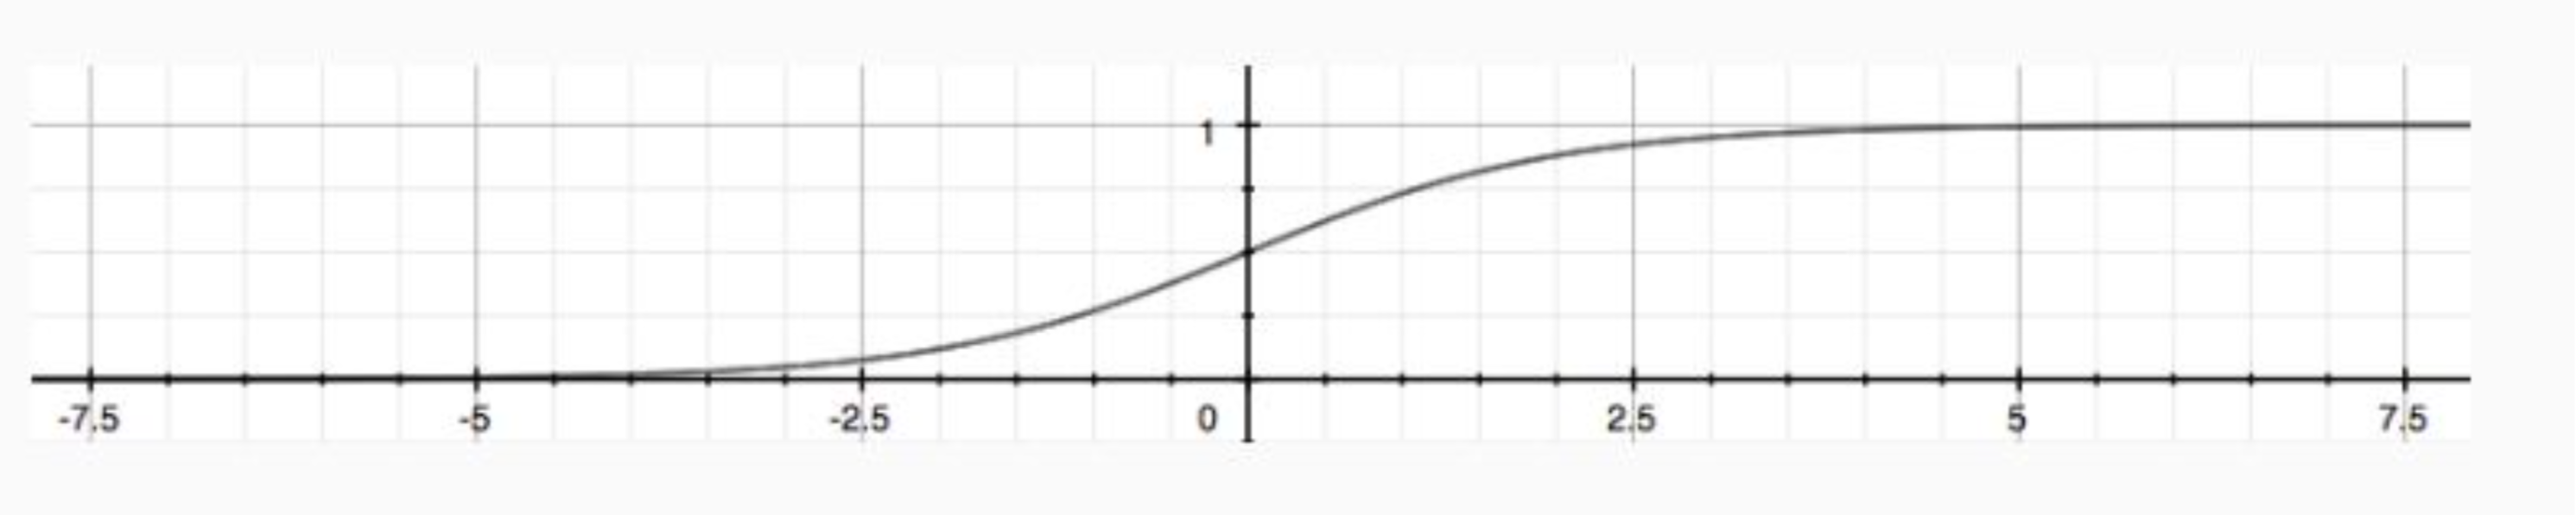
\includegraphics[width=150mm]{images/sigmoid_funct.png}}

The values of sigmoid function do not get bigger than 1 nor it gets lesser than 0. This is what makes it good for classification because our classification problem can only have values within the range (0,1).\\

Here’s the mathematical formula for it:\\

\centerline{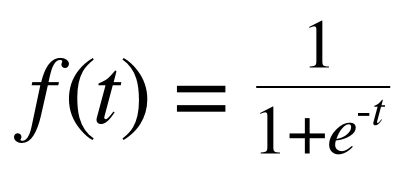
\includegraphics[width=75mm]{images/sigmoid_formula.png}}

\section*{Decision Boundary}

Decision boundary helps to differentiate probabilities into positive class and negative class. threshold value or tipping point above which we will classify values into class 1 and below which we classify values into class 2.\\

\centerline{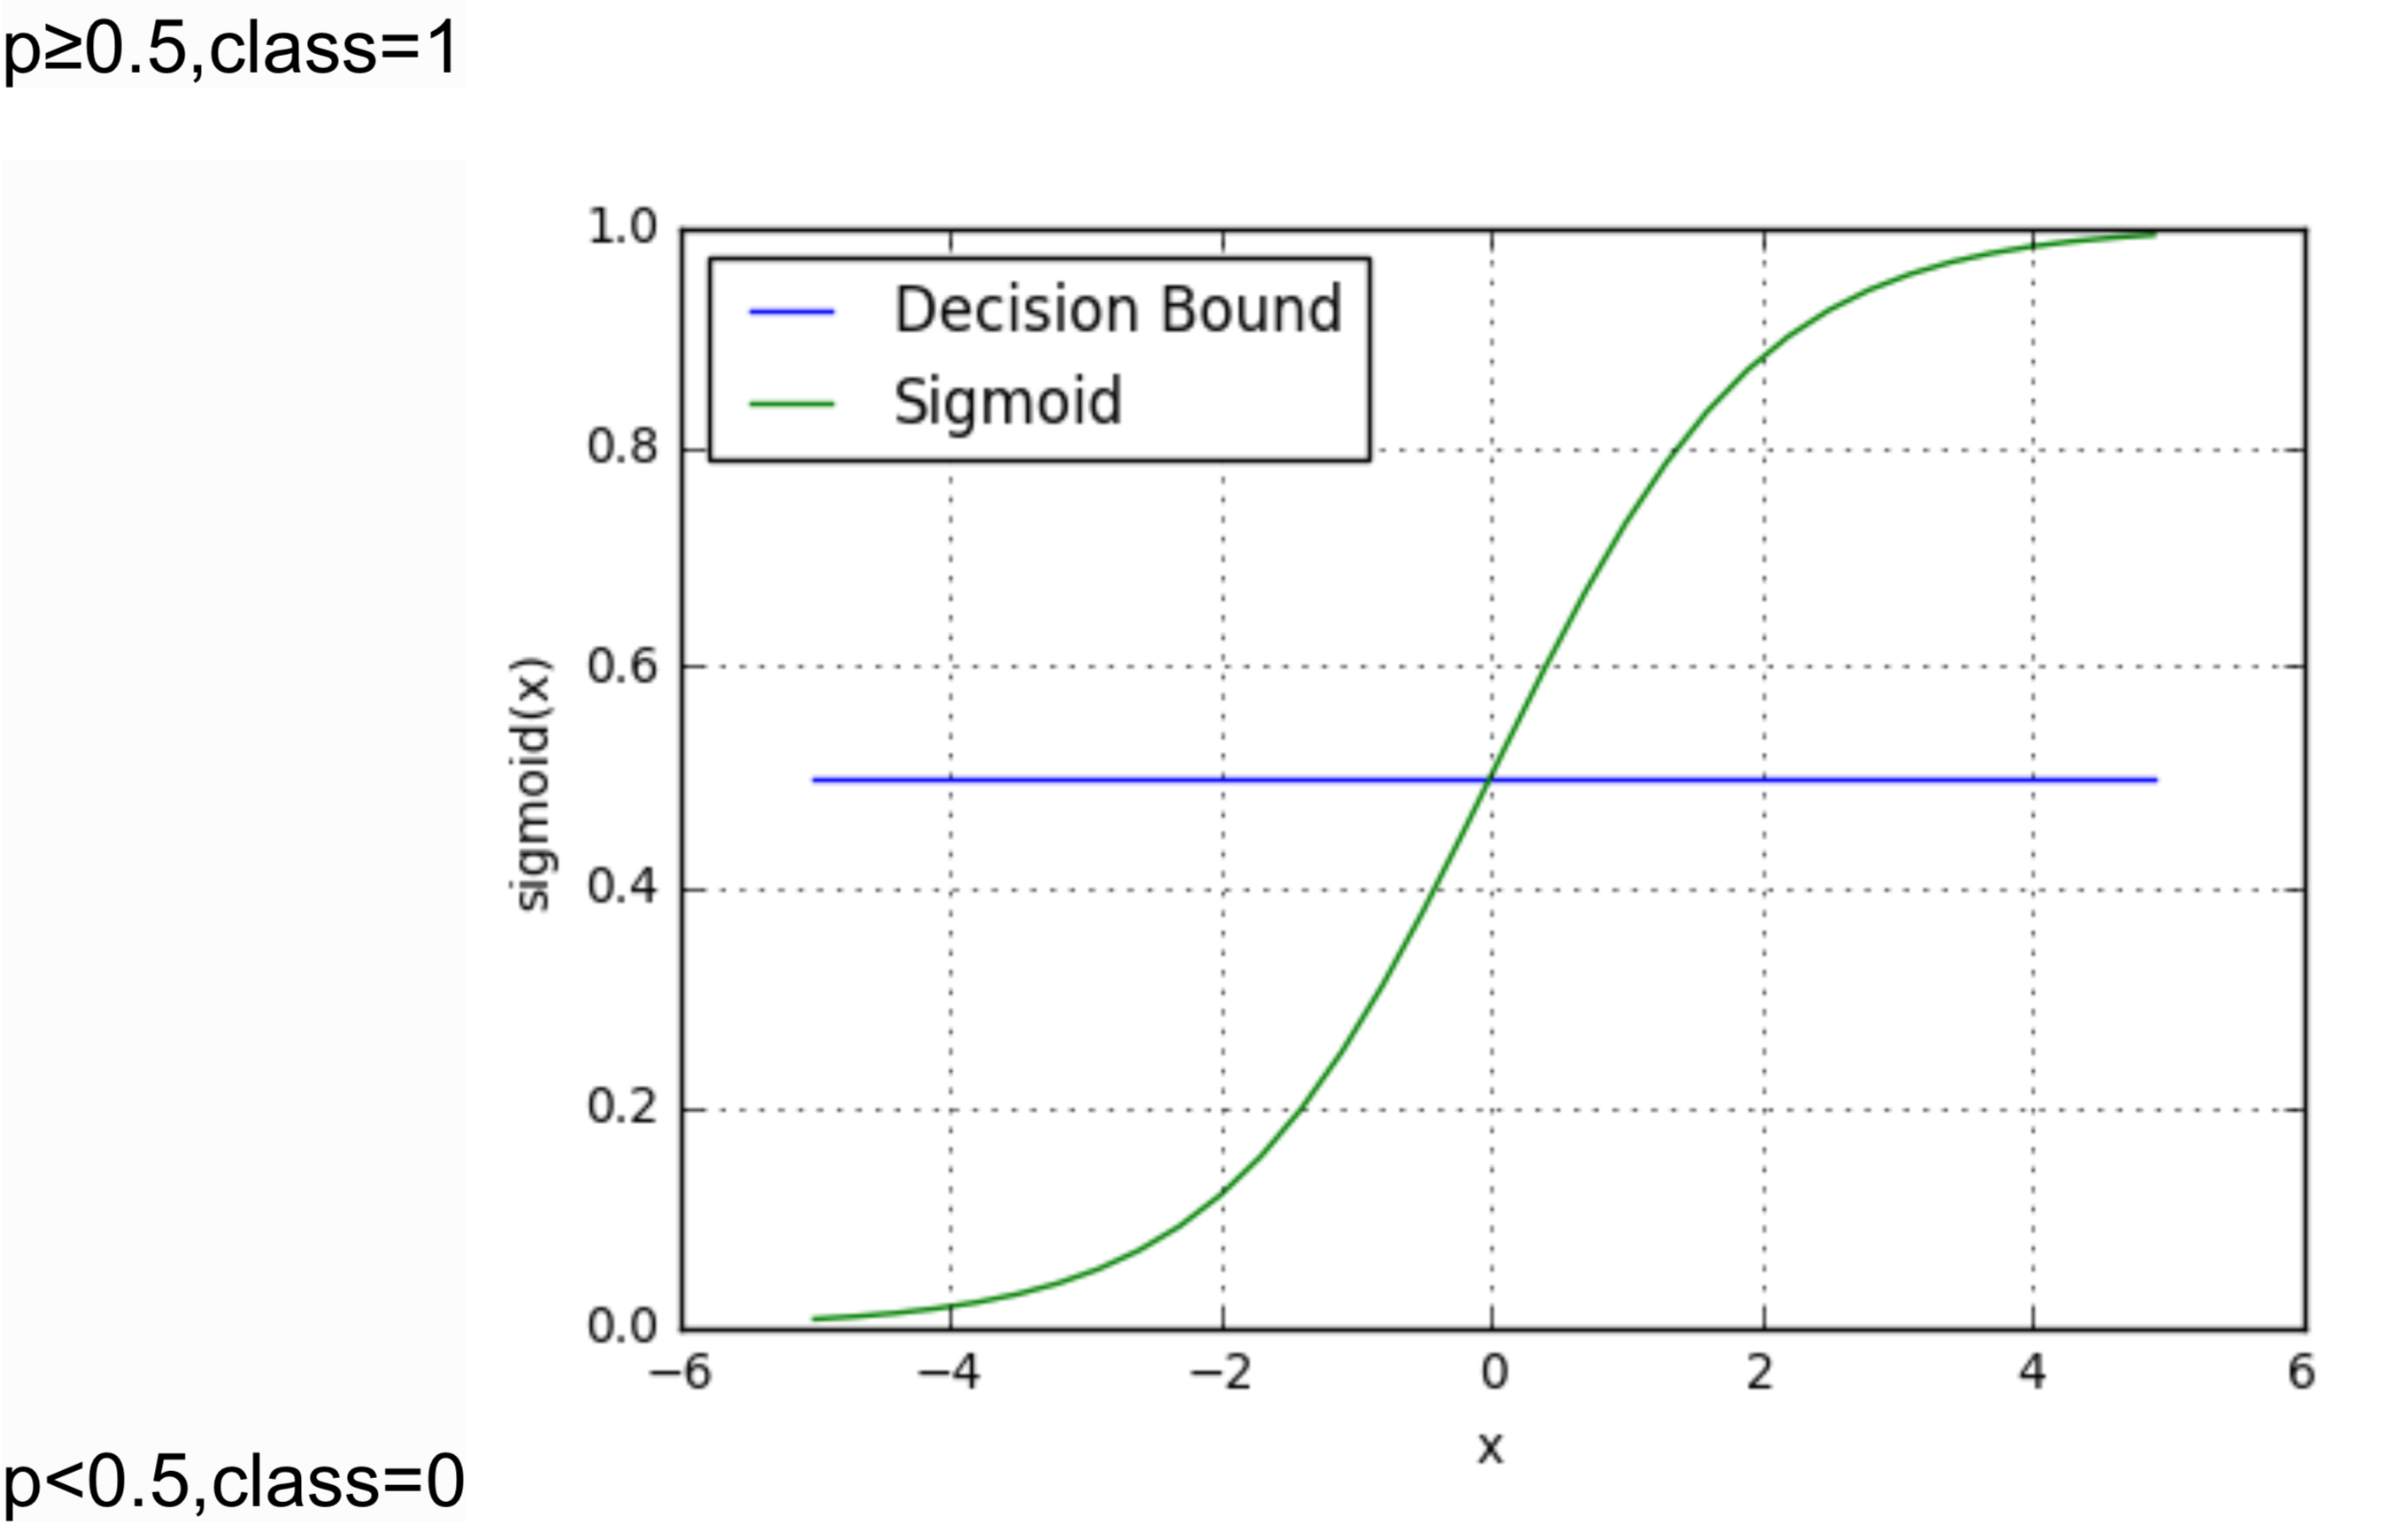
\includegraphics[width=150mm]{images/labelled_sigwthresh.png}}
\newpage
Linear Decision Boundary:\\

\centerline{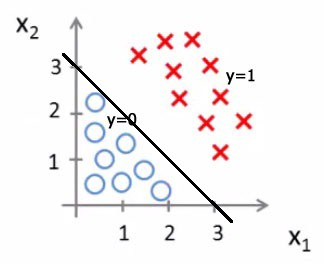
\includegraphics[width=75mm]{images/linear_db.jpeg}}

Non-linear Decision Boundary:\\

\centerline{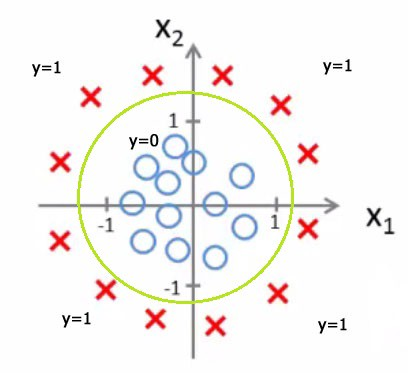
\includegraphics[width=75mm]{images/nonlinear_db.jpeg}}

\section*{Cost Function}

The cost function of logistic regression is not the same as the one we used for a linear regression. That’s because the logistic function will cause the output to have many local optima. In other words, it will not be a convex function.\\

\centerline{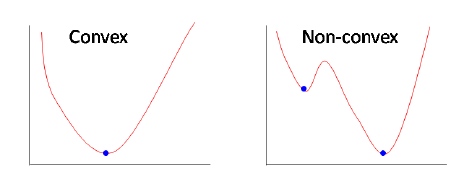
\includegraphics[width=150mm]{images/convnconv.png}}

What makes a non-convex optimization hard is the presence of saddle points and local minima, where the gradient is (0,...,0) and that have an arbitrarily bad objective value.\\

So instead, our cost function for logistic regression looks like:\\

\centerline{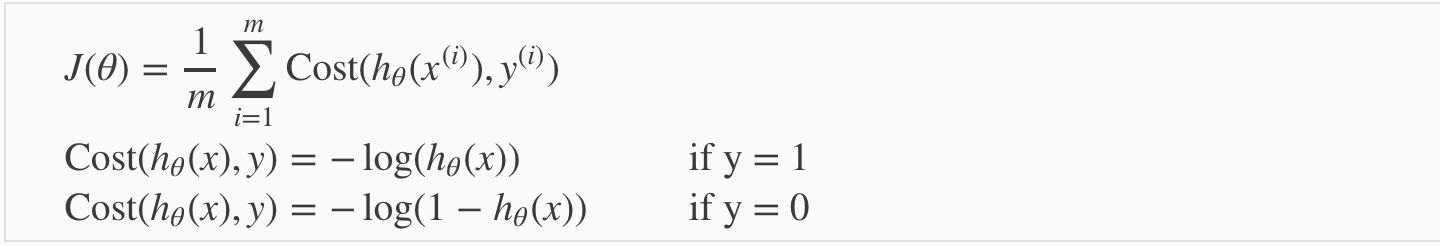
\includegraphics[width=150mm]{images/const_fun_log.png}}

In order to understand the above cost function in a better way, see the diagram below:\\

\centerline{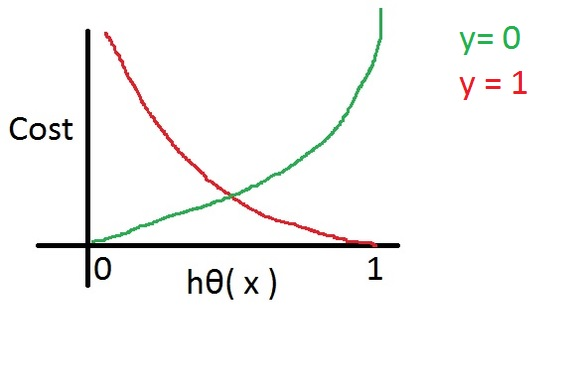
\includegraphics[width=75mm]{images/cost_draw.png}}

If our correct answer 'y' is 0, then the cost function will be 0 if our hypothesis function also outputs 0. If our hypothesis approaches 1, then the cost function will approach infinity.\\

If our correct answer 'y' is 1, then the cost function will be 0 if our hypothesis function outputs 1. If our hypothesis approaches 0, then the cost function will approach infinity.\\

Note that writing the cost function in this way guarantees that \(J(\theta)\) is convex for logistic regression.\\

\section*{More information!}
\begin{itemize}
    \item \href{https://towardsdatascience.com/machine-learning-classifiers-a5cc4e1b0623}{Machine Learning Classifiers}
    \item \href{https://www.youtube.com/watch?v=7qJ7GksOXoA}{Logistic Regression - Fun and Easy Machine Learning} (video)
    \item \href{https://medium.com/greyatom/logistic-regression-89e496433063}{Logistic Regression}
    \item The third week of \href{https://www.coursera.org/learn/machine-learning}{Andrew Ng’s Machine Learning course on Coursera}
\end{itemize}

%******************************************************************************%
%                                                                              %
%                               Ask your peers                                 %
%                                                                              %
%******************************************************************************%
\chapter{Ask Your Peers}

\begin{enumerate}
    \item Explain what classification is. What type of machine learning does it fall under?
    \item What is logistic regression? What is the function used for it?
    \item What is the difference between linear regression and logistic regression?
    \item Explain what is the use of the decision boundary.
    \item Why is the cost function used for logistic regression different from linear regression?
    \item What are the examples you can use a logistic function for?
    \item Besides logistic regressions, what are other classification models? List 3 of them.
\end{enumerate}

\startexercices


%******************************************************************************%
%                                                                              %
%                          Classification Project                              %
%                                                                              %
%******************************************************************************%

\chapter{Exercise 00: Classification Project}
\extopics{Logistic Regression, scikit-learn, pandas, numpy, matplotlib}
\turnindir{Logistic\_Regression}
\exfiles{suv\_launch\_prediction.py}
\extitle{Classification Project}
\makeheaderfiles

\section*{Scenario:}
Imagine that you’re a marketing associate for BMW, waiting for the working hour to end. Suddenly, you hear your boss knocking on your office door.\\
\texttt{\textbf{“Knock Knock”}\\
\textit{You open the door.}\\
Jeson (CEO): Hey, we are launching a new SUV next week and we need to create an Instagram ad to target people that will most likely buy the new SUV we are making.\\
You: Yes Jeson. I will get it done as soon as possible.\\}
The good news is you have the dataset of users who bought the previous model of SUV and you happen to know a little bit of machine learning (thanks to Hack High School).\\
Now, use logistic regression to classify and predict which customers would buy this new BMW SUV. You must be able to visualize the result by using the Matplotlib library. The image below is the end result of the test set that is expected to be displayed.\\
Using Jupyter notebook to build this project will be highly recommended. Download the dataset to begin. Happy hacking!\\

\hint{Use the \href{https://scikit-learn.org/stable/}{scikit-learn library} to perform feature scaling and logistic regression.}

\centerline{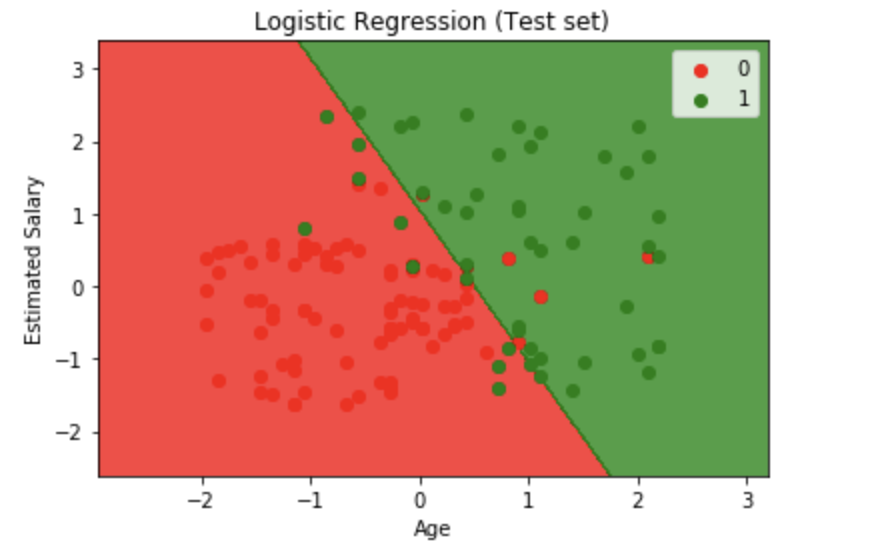
\includegraphics[width=100mm]{images/lr_testset.png}}

\nextexercice
\newpage

%******************************************************************************%
%                                                                              %
%                                 Bonuses                                      %
%                                                                              %
%******************************************************************************%

\chapter{Exercise 01: Bonus Project 1}
\extopics{Linear Regression, scikit-learn, pandas, numpy, matplotlib}
\turnindir{Bonus}
\exfiles{suv\_launch\_prediction\_1.py}
\extitle{Bonus Project 1}
\makeheaderfiles

Using the same dataset from the linear regression project, try performing other regression algorithms like support vector machine, decision tree regression or random forest regression and see the difference in them!\\
Work on at least 1 regression model other than linear regression.

\nextexercice
\newpage

\chapter{Exercise 02: Bonus Project 2}
\extopics{Logistic Regression, scikit-learn, pandas, numpy, matplotlib}
\turnindir{Bonus}
\exfiles{suv\_launch\_prediction\_2.py}
\extitle{Bonus Project 2}
\makeheaderfiles

Using the same dataset from the logistic regression project, try performing other classification algorithms like K-Nearest-Neighbors, naive bayes, decision tree classification or random forest classification and see the difference in them!\\
Work on at least 1 classification model other than logistic regression.

\nextexercice
\newpage

% %******************************************************************************%
% %                                                                              %
% %                                   Conclusion                                 %
% %                                                                              %
% %******************************************************************************%

 \chapter{Conclusion}

I hope this course gave you a basic understanding and fundamentals of machine learning. You have learned the essential python libraries through exercises to building your own machine learning model. I hope you enjoyed what we have put together and use the skills to further improve yourself.\\
If you like this course, I will try to work on creating a more advanced course called “intro to deep learning” where you will learn about neural network and eventually creating something really cool that you can show off to your classmates.\\
Please fill out \href{https://goo.gl/forms/PcRd7YRTuRPBDFKx2}{this feedback form here} to let me know what you think about the course and what I can improve.
\section*{References and image sources:}
\begin{itemize}
    \item \href{https://towardsdatascience.com/}{Towards Data Science}
    \item \href{https://www.udemy.com/machinelearning/}{Udemy course (Machine Learning A to Z)}
    \item \href{https://hackernoon.com/}{Hackernoon}
    \item \href{https://www.machinelearningplus.com/}{Machine Learning Plus}
    \item \href{https://www.coursera.org/courses?query=machine\%20learning\%20stanford}{Coursera Stanford Machine Learning course}
    \item \href{https://www.kaggle.com/}{Kaggle}
\end{itemize}

\end{document}